\documentclass[10pt,a4paper]{article}

\usepackage[a4paper,margin=22mm,headheight=14pt]{geometry}
\usepackage[UTF8]{ctex}
\usepackage{amsmath,amssymb}
\usepackage{booktabs}
\usepackage{longtable}
\usepackage{seqsplit}
\usepackage{graphicx}
\usepackage{microtype}
\usepackage{xcolor}
\usepackage{caption}
\usepackage{pdflscape}
\usepackage[numbers,sort&compress]{natbib}
\usepackage{fancyhdr}
\usepackage[hidelinks]{hyperref}

\definecolor{navy}{HTML}{214B6B}
\hypersetup{colorlinks=true,linkcolor=navy,citecolor=navy,urlcolor=navy}
\captionsetup{font=small,labelfont={bf,color=navy},justification=justified,hypcap=false}
\graphicspath{{figures/}}
\pagestyle{fancy}
\fancyhf{}
\fancyhead[L]{\small SafeEdit-CRE 补充信息}
\fancyhead[R]{\small 调控基因组学与序列设计}
\fancyfoot[C]{\thepage}

\title{\textbf{补充信息}\\[0.35em]
\large 跨模型不确定性感知的顺式调控元件最小编辑：细胞类型选择性设计}
\author{夏昂然\\
陕西师范大学化学化工学院\\
陕西省西安市长安区西长安街620号 710119\\[0.35em]
\textit{通信邮箱：} \texttt{haangyeon@snnu.edu.cn}}
\date{}

\begin{document}
\maketitle
\tableofcontents
\clearpage

\section{补充方法与审计说明}

\subsection{研究阶段与角色分离}

本研究按序贯阶段执行。G0--G3建立了数据审计、已发表模型重现、试点CNN评审器以及初始编辑工作流。G4冻结了90亲本、三方法的硬性审计基准（6个名义亲本因与G4探索性试点重叠而被排除）。G6分配了计算候选层级。G7训练了全数据残基-扩张评审器和多核冻结后评估器。G8选择了600个新亲本并比较了四种搜索方法。G9在180个亲本上重运行了七种完整搜索配置。G10应用了冻结后终点并组装了汇总分析。活性标签从未用于选择亲本或候选序列。

术语\emph{评审器}和\emph{冻结后评估器}表示不同的角色。评审器在G8/G9搜索期间可供SafeEdit使用。冻结后评估器仅在候选文件冻结后才加载。两者均在相同的公开MPRA源表上训练；因此"冻结后"描述的是与搜索的程序分离，而非外部生物学独立性。

\subsection{完整性检查}

最终G9表包含15,120行、180个唯一条本、七种配置、三个靶细胞和四个预算。不存在重复的亲本--靶标--预算--配置键，无非有限数值，可行设计中无精确编辑预算违规。G8折叠表包含28,800行方法级记录和600个亲本。随机指标是三次独立重复的均值；折叠表不得用于选择特定DNA序列。

所有投稿载荷均在手稿生成后重新检查。发布清单包含每个载荷文件的SHA-256校验和，且清单本身不参与自哈希计算。

\section{补充结果}

\subsection{数据划分与预测器性能}

\begin{table}[ht]
\centering
\caption{\textbf{表S1。} 用于G7模型训练的质量过滤后全数据划分。}
\label{tab:S1}
{\small
\begin{tabular}{lrrp{4.5cm}}
\toprule
划分 & 记录数 & 染色体 & 用途 \\
\midrule
训练集 & 627,661 & 排除验证/测试的符合条件染色体 & 参数拟合 \\
验证集 & 58,811 & 19、21、X & 检查点选择和方差缩放 \\
测试集 & 62,582 & 7、13 & 最终预测诊断 \\
\midrule
总计 & 749,054 & -- & 质量过滤和精确去重后 \\
\bottomrule
\end{tabular}
}
\end{table}

\begin{table}[ht]
\centering
\caption{\textbf{表S2。} 62,582条记录测试拆分上的集成性能，从保存的候选独立预测表重新计算。}
\label{tab:S2}
\begin{tabular}{llrrrr}
\toprule
模型 & 细胞 & Pearson $r$ & Spearman $\rho$ & MAE & 不确定性--误差 $\rho$ \\
\midrule
评审器 & K562 & 0.845 & 0.781 & 0.396 & 0.448 \\
评审器 & HepG2 & 0.855 & 0.809 & 0.354 & 0.404 \\
评审器 & SK-N-SH & 0.847 & 0.810 & 0.390 & 0.399 \\
\addlinespace
冻结后评估器 & K562 & 0.785 & 0.719 & 0.463 & 0.467 \\
冻结后评估器 & HepG2 & 0.795 & 0.743 & 0.417 & 0.416 \\
冻结后评估器 & SK-N-SH & 0.799 & 0.760 & 0.444 & 0.400 \\
\bottomrule
\end{tabular}
\end{table}

\begin{table}[ht]
\centering
\caption{\textbf{表S3。} 测试拆分上的验证缩放区间覆盖率。}
\label{tab:S3}
\begin{tabular}{llrrr}
\toprule
模型 & 细胞 & 80\%区间 & 90\%区间 & 95\%区间 \\
\midrule
评审器 & K562 & 0.815 & 0.897 & 0.935 \\
评审器 & HepG2 & 0.794 & 0.885 & 0.930 \\
评审器 & SK-N-SH & 0.814 & 0.900 & 0.940 \\
\addlinespace
冻结后评估器 & K562 & 0.821 & 0.900 & 0.935 \\
冻结后评估器 & HepG2 & 0.789 & 0.879 & 0.923 \\
冻结后评估器 & SK-N-SH & 0.816 & 0.899 & 0.935 \\
\bottomrule
\end{tabular}
\end{table}

\begin{figure}[ht]
\centering
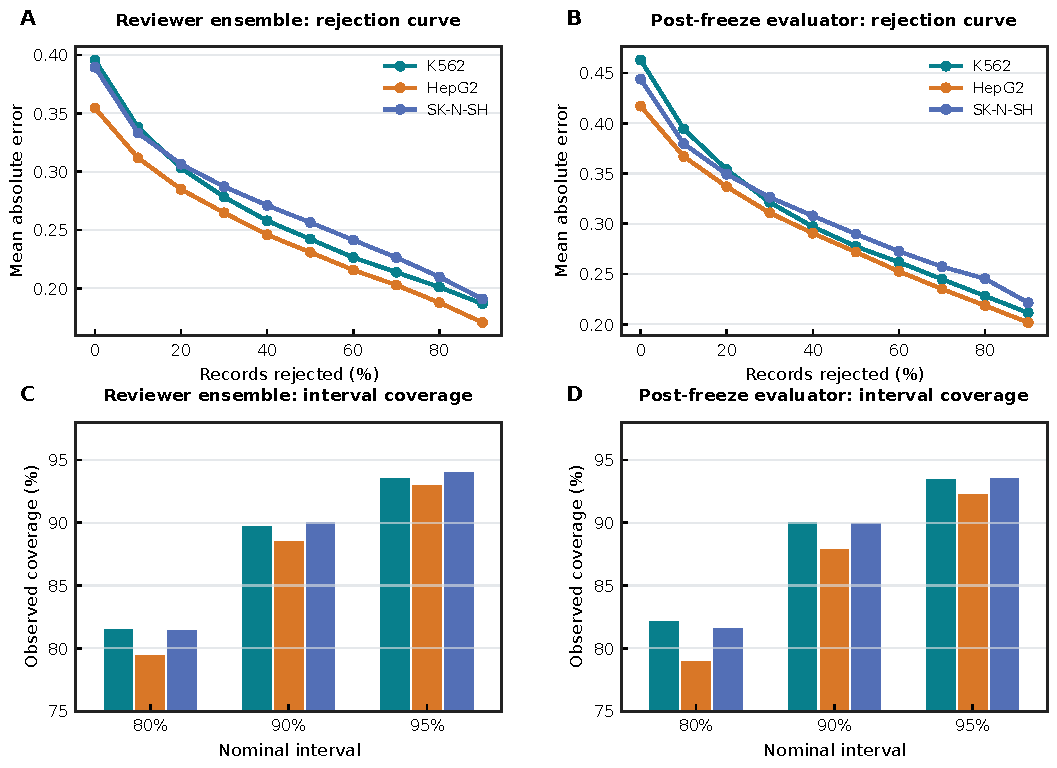
\includegraphics[width=\textwidth]{figS1_uncertainty_rejection.pdf}
\caption{\textbf{图S1。不确定性拒绝与区间校准。} \textbf{A--B}，随着预测不确定性最大的记录从留出测试集中移除，评审器和冻结后集成的平均绝对误差变化。\textbf{C--D}，按细胞类型划分的80\%、90\%和95\%名义水平下的观测测试覆盖率。曲线和柱状图为描述性测试诊断；方差尺度仅从验证集固定。}
\label{fig:S1}
\end{figure}

\clearpage
\subsection{G4硬性审计分层}

\begin{longtable}{llrrrr}
\caption{\textbf{表S4。} 按靶细胞和编辑预算划分的G4审计通过率。每行包含90个非重叠亲本/方法，排除了6个与G4探索性试点重叠的亲本。}\label{tab:S4}\\
\toprule
靶标 & 预算 & 随机(\%) & 贪婪(\%) & SafeEdit(\%) & SafeEdit--贪婪(pp) \\
\midrule
\endfirsthead
\toprule
靶标 & 预算 & 随机(\%) & 贪婪(\%) & SafeEdit(\%) & SafeEdit--贪婪(pp) \\
\midrule
\endhead
K562 & 1 & 14.4 & 58.9 & 60.0 & 1.1 \\
K562 & 5 & 8.9 & 56.7 & 77.8 & 21.1 \\
K562 & 10 & 17.8 & 43.3 & 82.2 & 38.9 \\
K562 & 20 & 24.4 & 50.0 & 81.1 & 31.1 \\
HepG2 & 1 & 8.9 & 34.4 & 35.6 & 1.1 \\
HepG2 & 5 & 5.6 & 35.6 & 45.6 & 10.0 \\
HepG2 & 10 & 2.2 & 33.3 & 56.7 & 23.3 \\
HepG2 & 20 & 8.9 & 27.8 & 60.0 & 32.2 \\
SK-N-SH & 1 & 24.4 & 36.7 & 38.9 & 2.2 \\
SK-N-SH & 5 & 17.8 & 35.6 & 57.8 & 22.2 \\
SK-N-SH & 10 & 15.6 & 22.2 & 64.4 & 42.2 \\
SK-N-SH & 20 & 8.9 & 31.1 & 66.7 & 35.6 \\
\bottomrule
\end{longtable}

\subsection{G8冻结后终点与异质性}

\begin{table}[ht]
\centering
\caption{\textbf{表S5。} 合并的G8方法汇总。每种方法在三次随机重复取平均后有7,200条亲本--靶标--预算记录。}
\label{tab:S5}
\begin{tabular}{lrrrr}
\toprule
方法 & 裕度增益 & 靶标增益 & 正裕度比例(\%) & 不确定性 \\
\midrule
随机匹配 & 0.001 & 0.012 & 48.6 & 0.185 \\
贪婪Malinois & 0.822 & 1.803 & 97.1 & 0.329 \\
主束 & 0.881 & 1.866 & 94.8 & 0.335 \\
SafeEdit共识 & 0.877 & 1.661 & 95.4 & 0.314 \\
\bottomrule
\end{tabular}
\end{table}

\begin{table}[ht]
\centering
\caption{\textbf{表S6。} 合并的配对G8对比。差值为SafeEdit减去对照；置信区间使用100,000次亲本簇自助重复。}
\label{tab:S6}
\begin{tabular}{llrr}
\toprule
对照 & 指标 & 平均差值 & 95\% CI \\
\midrule
贪婪 & 冻结后裕度增益 & 0.0555 & 0.0398 至 0.0705 \\
贪婪 & 冻结后靶标增益 & $-0.1412$ & $-0.1774$ 至 $-0.1057$ \\
贪婪 & 冻结后不确定性 & $-0.0153$ & $-0.0214$ 至 $-0.0091$ \\
\addlinespace
主束 & 冻结后裕度增益 & $-0.0036$ & $-0.0114$ 至 0.0042 \\
主束 & 冻结后靶标增益 & $-0.2048$ & $-0.2294$ 至 $-0.1808$ \\
主束 & 冻结后不确定性 & $-0.0209$ & $-0.0251$ 至 $-0.0166$ \\
\addlinespace
随机匹配 & 冻结后裕度增益 & 0.8763 & 0.8562 至 0.8960 \\
随机匹配 & 冻结后靶标增益 & 1.6494 & 1.6034 至 1.6950 \\
随机匹配 & 冻结后不确定性 & 0.1285 & 0.1222 至 0.1348 \\
\bottomrule
\end{tabular}
\end{table}

\clearpage
\begin{center}
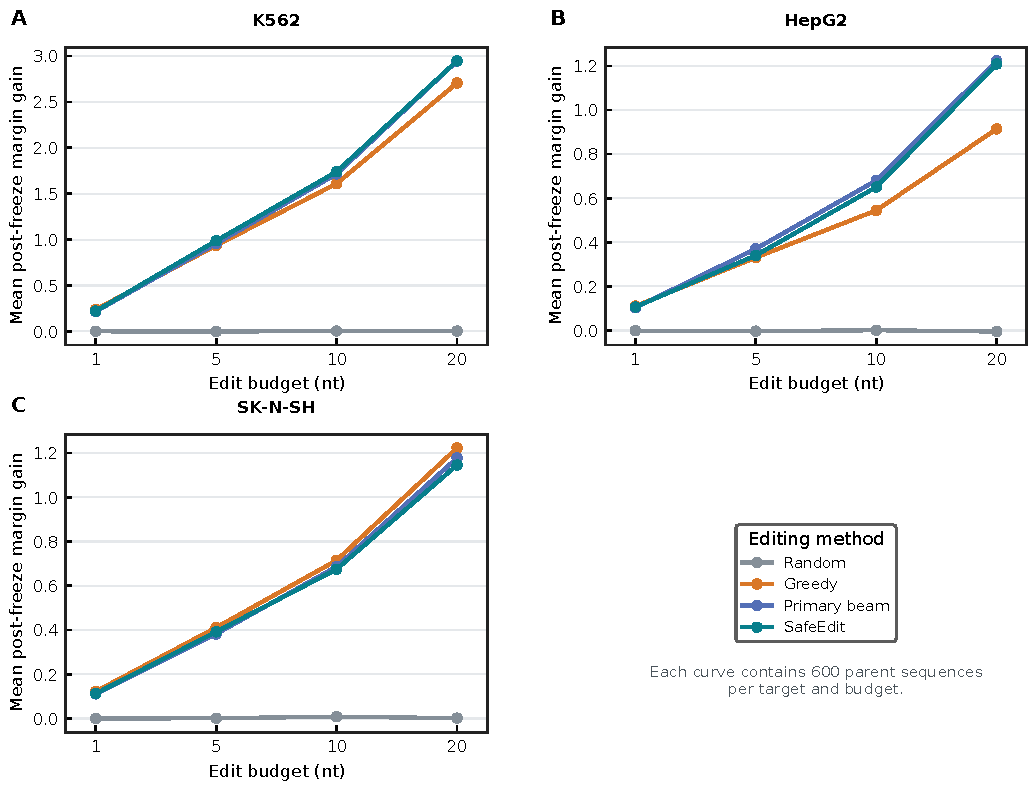
\includegraphics[width=0.96\textwidth]{figS2_stratified_effects.pdf}
\captionof{figure}{\textbf{图S2。G8冻结后终点中的靶标--预算异质性。}
\textbf{A--C}，K562、HepG2和SK-N-SH中随机、贪婪、主束和SafeEdit搜索在不同编辑预算下的平均冻结后特异性裕度增益。每个点汇总600个亲本。数值为描述性，未做多重性校正。}
\label{fig:S2}
\end{center}

\clearpage
\subsection{G9真实搜索消融}

\begin{table}[ht]
\centering
\caption{\textbf{表S7。} 七种独立重运行搜索配置的G9冻结后结果。每种配置包含2,160行，来自180个亲本、三个靶标和四个预算。}
\label{tab:S7}
\begin{tabular}{lrrrrr}
\toprule
配置 & 裕度增益 & 靶标增益 & 正例比例(\%) & 不确定性 & 不可行 \\
\midrule
主束 & 0.890 & 1.897 & 94.7 & 0.334 & 48 \\
SafeEdit完整 & 0.890 & 1.705 & 95.3 & 0.312 & 48 \\
无评审得分 & 0.890 & 1.897 & 94.7 & 0.334 & 48 \\
无不确定性惩罚 & 0.891 & 1.719 & 95.2 & 0.313 & 48 \\
无链惩罚 & 0.887 & 1.701 & 95.4 & 0.310 & 48 \\
无天然性重排序 & 0.979 & 2.017 & 95.3 & 0.343 & 48 \\
无序列预过滤器 & 0.910 & 1.763 & 98.1 & 0.318 & 0 \\
\bottomrule
\end{tabular}
\end{table}

\begin{table}[ht]
\centering
\caption{\textbf{表S8。} 选定的G9配对对比。差值为完整SafeEdit减去消融配置；区间使用100,000次亲本簇自助重复。}
\label{tab:S8}
\begin{tabular}{llrr}
\toprule
对照 & 指标 & 平均差值 & 95\% CI \\
\midrule
主束 & 冻结后裕度增益 & 0.0002 & $-0.0145$ 至 0.0151 \\
主束 & 冻结后靶标增益 & $-0.1920$ & $-0.2440$ 至 $-0.1432$ \\
主束 & 冻结后不确定性 & $-0.0212$ & $-0.0283$ 至 $-0.0140$ \\
\addlinespace
无天然性 & 冻结后裕度增益 & $-0.0888$ & $-0.1022$ 至 $-0.0754$ \\
无天然性 & 冻结后靶标增益 & $-0.3117$ & $-0.3600$ 至 $-0.2658$ \\
无天然性 & 冻结后不确定性 & $-0.0305$ & $-0.0394$ 至 $-0.0218$ \\
\addlinespace
无预过滤器 & 冻结后裕度增益 & $-0.0198$ & $-0.0387$ 至 $-0.0043$ \\
无预过滤器 & 冻结后靶标增益 & $-0.0581$ & $-0.1021$ 至 $-0.0227$ \\
无预过滤器 & 冻结后不确定性 & $-0.0060$ & $-0.0102$ 至 $-0.0024$ \\
\bottomrule
\end{tabular}
\end{table}

\subsection{候选文库}

\clearpage
\begin{center}

\includegraphics[width=0.86\textwidth]{figS3_candidate_tiers.pdf}
\captionof{figure}{\textbf{图S3。计算候选层级。} 冻结的3,240条序列G4文库的主模型和评审特异性裕度增益。所有Tier A和Tier B候选均被绘制；Tier C为可读性进行了降采样。带轮廓的点位于计算的帕累托前沿上。层级标签表示实验筛选的计算优先级。}
\label{fig:S3}
\end{center}

\begin{table}[ht]
\centering
\caption{\textbf{表S9。} 冻结的G4候选层级。}
\label{tab:S9}
\begin{tabular}{lrrl}
\toprule
层级 & 候选数 & 比例(\%) & 预期用途 \\
\midrule
A & 74 & 2.3 & 最高优先级实验组 \\
B & 1,141 & 35.2 & 备选计算候选 \\
C & 2,025 & 62.5 & 方法与失效模式分析 \\
\bottomrule
\end{tabular}
\end{table}

\subsection{代表性Tier A候选}

\begin{landscape}
\begin{longtable}{p{2.2cm}p{2.0cm}p{2.0cm}p{2.0cm}p{2.0cm}p{2.0cm}p{2.0cm}}
\caption{\textbf{表S10。} 三个代表性Tier A报告基因筛选候选，每种细胞类型一个，选自锁定的非重叠90亲本九准则设计基准。代表性示例按预设规则选择：要求Tier A状态、每种靶细胞一个示例、正的跨模型裕度增益、降低的不确定性、无合成风险标记。裕度显示主Malinois预测器和留出评审集成的结果；三者均达到帕累托前沿状态且无合成风险标记。编辑位置使用200-nt序列窗口内的0索引坐标。裕度和不确定性值以log倍变化单位表示。GC以分数表示。所有编辑均为5个核苷酸预算内的替换。编辑位置的基序水平观测作为可检验的序列语法假说报告，供后续研究。}\label{tab:S10}\\
\toprule
属性 & \multicolumn{2}{c}{K562 (chr7:127284707)} & \multicolumn{2}{c}{HepG2 (chr7:105701659)} & \multicolumn{2}{c}{SK-N-SH (chr13:23368564)} \\
\cmidrule(lr){2-3}\cmidrule(lr){4-5}\cmidrule(lr){6-7}
& 亲本 & 编辑后 & 亲本 & 编辑后 & 亲本 & 编辑后 \\
\midrule
\endfirsthead
\toprule
属性 & K562亲本 & K562编辑 & HepG2亲本 & HepG2编辑 & SK-N-SH亲本 & SK-N-SH编辑 \\
\midrule
\endhead
编辑预算 & \multicolumn{2}{c}{5} & \multicolumn{2}{c}{5} & \multicolumn{2}{c}{5} \\
编辑位置 & \multicolumn{2}{c}{\small 89, 118, 130, 132, 180} & \multicolumn{2}{c}{\small 89, 94, 99, 112, 199} & \multicolumn{2}{c}{\small 1, 148, 149, 171, 174} \\
编辑详情 & \multicolumn{2}{c}{\small 89T>A; 118C>G; 130A>T; 132C>A; 180C>A} & \multicolumn{2}{c}{\small 89G>T; 94C>A; 99G>C; 112G>C; 199C>G} & \multicolumn{2}{c}{\small 1C>G; 148T>C; 149C>T; 171A>G; 174C>A} \\
\addlinespace
主裕度 & $-0.372$ & $+4.204$ & $-0.620$ & $+5.100$ & $+0.020$ & $+2.874$ \\
评审裕度 & $-0.138$ & $+0.002$ & $-0.068$ & $+0.003$ & $-0.197$ & $-0.097$ \\
主裕度增益 & \multicolumn{2}{c}{$+4.577$} & \multicolumn{2}{c}{$+5.719$} & \multicolumn{2}{c}{$+2.854$} \\
评审裕度增益 & \multicolumn{2}{c}{$+0.140$} & \multicolumn{2}{c}{$+0.070$} & \multicolumn{2}{c}{$+0.100$} \\
主靶标增益 & \multicolumn{2}{c}{$+4.558$} & \multicolumn{2}{c}{$+6.093$} & \multicolumn{2}{c}{$+3.427$} \\
评审不确定性 & $1.253$ & $1.099$ & $1.243$ & $1.143$ & $0.552$ & $0.445$ \\
不确定性变化 & \multicolumn{2}{c}{$-0.154$} & \multicolumn{2}{c}{$-0.100$} & \multicolumn{2}{c}{$-0.107$} \\
\addlinespace
GC含量 & $0.575$ & $0.565$ & $0.570$ & $0.560$ & $0.365$ & $0.365$ \\
天然性变化 & \multicolumn{2}{c}{$+0.056$} & \multicolumn{2}{c}{$+0.006$} & \multicolumn{2}{c}{$+0.028$} \\
最大同源多聚体 & $4$ & $4$ & $5$ & $5$ & $5$ & $5$ \\
合成风险 & \multicolumn{2}{c}{无} & \multicolumn{2}{c}{无} & \multicolumn{2}{c}{无} \\
帕累托前沿 & \multicolumn{2}{c}{是} & \multicolumn{2}{c}{是} & \multicolumn{2}{c}{是} \\
\addlinespace
亲本序列 & \multicolumn{6}{p{22.8cm}}{\ttfamily\scriptsize\seqsplit{TGAGGGCAGAGCTCAGCCGCAACCCGGCCCTGCTGCTTAGAGGCTCGGGGCCTTGGCAAATGACAGCCTCCCTGAGCCTGTTTCTCCATCCGTAAAACAGGCCTCCCAGCCCTGTGTCGGAGCAACTGAAACGAGGGTTAAATGAGGAAACCATGCGACAGATGTCAGCATAATCCCTGCCACGCAGAGGAGGCAAAATC}} \\
编辑后序列(K562) & \multicolumn{6}{p{22.8cm}}{\ttfamily\scriptsize\seqsplit{TGAGGGCAGAGCTCAGCCGCAACCCGGCCCTGCTGCTTAGAGGCTCGGGGCCTTGGCAAATGACAGCCTCCCTGAGCCTGTTTCTCCAACCGTAAAACAGGCCTCCCAGCCCTGTGTGGGAGCAACTGATAAGAGGGTTAAATGAGGAAACCATGCGACAGATGTCAGCATAATCCCTGACACGCAGAGGAGGCAAAATC}} \\
\addlinespace
亲本序列(HepG2) & \multicolumn{6}{p{22.8cm}}{\ttfamily\scriptsize\seqsplit{GGGGGTGAGGGATCCCTGCAATACATAACACGTGCTAAGCAGTGGGGTTTGGGTGCTACTTCCCAACTGGCCGCTCTTAGGAACTGGTGAAACCTTAAGTCAGGTGTGACTGAGCGAGCCCCTGGGTCATGGCTATTCTCCTTGCTGCTCTGCTCTCCTAAGTCTGGTTTGAGGCTCCTCTCCCTCCCTGGCGTCCCACC}} \\
编辑后序列(HepG2) & \multicolumn{6}{p{22.8cm}}{\ttfamily\scriptsize\seqsplit{GGGGGTGAGGGATCCCTGCAATACATAACACGTGCTAAGCAGTGGGGTTTGGGTGCTACTTCCCAACTGGCCGCTCTTAGGAACTGGTTAAACATTAACTCAGGTGTGACTCAGCGAGCCCCTGGGTCATGGCTATTCTCCTTGCTGCTCTGCTCTCCTAAGTCTGGTTTGAGGCTCCTCTCCCTCCCTGGCGTCCCAGC}} \\
\addlinespace
亲本序列(SK-N-SH) & \multicolumn{6}{p{22.8cm}}{\ttfamily\scriptsize\seqsplit{CGAAATTCCCACAACTGGAATATATACCGCATTGATACTATCTTCCCCTTTATCCTAAAACTGTCATCTTTAAGCTTCAAACAGTACTGTGATTTGATGTTAACCATGATGATTTGTACAACCGTATTTACAAGGCCACAACTCAAGTCATTTTTAGATTTCATCCTTCTAGACTGTAGCCAAATTCCCATCCATAAAGC}} \\
编辑后序列(SK-N-SH) & \multicolumn{6}{p{22.8cm}}{\ttfamily\scriptsize\seqsplit{GGAAATTCCCACAACTGGAATATATACCGCATTGATACTATCTTCCCCTTTATCCTAAAACTGTCATCTTTAAGCTTCAAACAGTACTGTGATTTGATGTTAACCATGATGATTTGTACAACCGTATTTACAAGGCCACAACTCAAGCTATTTTTAGATTTCATCCTTCTGGAATGTAGCCAAATTCCCATCCATAAAGC}} \\
\midrule[\heavyrulewidth]
\multicolumn{7}{p{23.4cm}}{\footnotesize 注：P = 亲本天然CRE；E = SafeEdit-CRE编辑设计。主裕度和靶标增益来自用于指导搜索的Malinois预测器；评审裕度和不确定性来自用于跨模型重排序的独立残基-扩张集成。所有编辑后序列保持长度200 nt和精确编辑预算。包含74个候选的完整Tier A文库作为机器可读表格提供在冻结发布包中。} \\
\bottomrule
\end{longtable}
\end{landscape}

\clearpage
\section{可重复性总结}

亲本选择是确定性的且标签盲的，在构建基准前移除了所有历史标识符、序列哈希和审计标记的冲突。冻结后评估器仅在候选文件及其SHA-256清单写入后才加载。计算量匹配的束使用与SafeEdit相同的束宽、扩展深度和预筛选大小；随机比较取三次固定重复的平均。最终置信区间使用100,000次亲本簇自助重复。所有七种消融配置均重运行了完整搜索，每张报告的图和表均可从分析脚本附带的候选级数据重新生成。

\end{document}
